\newpage
\subsubsection{Review 1}
\begin{tabularx}{\textwidth}{l|X|X}
\textbf{ID} & \textbf{Original Text} & \textbf{Preprocessed Text}\\
\hline
7894 &
In this film I prefer Deacon Frost. He\'s so sexy! I love his glacial eyes! I like Stephen Dorff and the vampires, so I went to see it. I hope to see a gothic film with him. "Blade" it was very "about the future". If vampires had been real, I would be turned by Frost!
&
film prefer deacon frost he sexi love glacial eye like stephen dorff vampir went see hope see gothic film blade futur vampir real would turn frost
\end{tabularx}

\begin{figure}[htb!]
	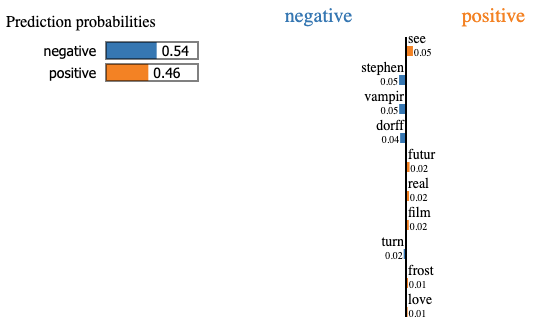
\includegraphics[width=\textwidth]{img/review_1}
	\caption{Wrongly classified review 1}
\end{figure}
\textbf{Reasons for wrong classification:}

As we see here in the original there was talk about vampires which is seen as a negative thing (which technically is true for horror movies etc.),but in this case it was actually a positive review but the positive words don't outweigh the negative ones.
So that the review got wrongly classified as negative